\section{Analysis}
\label{sec:auswertung}

\subsection{Theta-squared plot and detector significance}
After applying the event selection descriped in the implementation, the on- and off-events are 
displayed to find a cut-off value. 
The theta-squared plot for the selected data as well as the cut-off is shown in Figure \ref{fig:onoff}.

\begin{figure}[H]
  \centering
  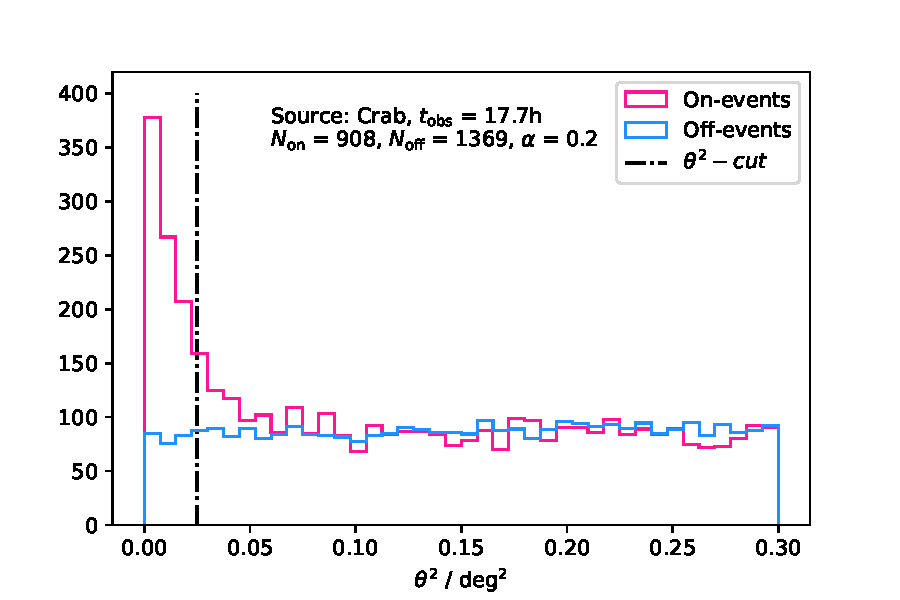
\includegraphics[width=0.8\textwidth]{plots/On_Off2.pdf}
  \caption{theta-squared plot for on-region and off-region data.}
  \label{fig:onoff}
\end{figure}

It can be seen, that the off-region events are evenly distributed throughout the entire angular space and the on-region events peak at small distances to the source, as expected.

The detector-significance for the given parameters in Figure \ref{fig:onoff} results in
\begin{equation}
  S = 26.2759\,.
\end{equation}
Futher evaluation is needed to determine weather this value is adequate.

\subsection{Migration matrix and unfolding}
To calculate the migration matrix, the estimated values \texttt{gamma\_energy\_prediction} of the \texttt{gamma\_test\_dl3\.hdf5} 
sample and the true-values \texttt{corsika\_event\_header\_total\_energy} are used.
The inverse problem is better conditioned if the binning is made with regards to the measured parameter, not in the unfolded.
Therefore the bins range from $\SI{500}{\giga\electronvolt}$ to $\SI{15}{\tera\electronvolt}$ in a logarithmic scale. 
An extra bin at $\SI{50}{\tera\electronvolt}$ is established to catch events wth a higher energy than the upper threshold.
This was done for both the estimated and the true values. The normed migration matrix is shown in Figure \ref{fig:matrix}.

It can be seen, that the correlation is quite close to one.
\begin{figure}[H]
  \centering
  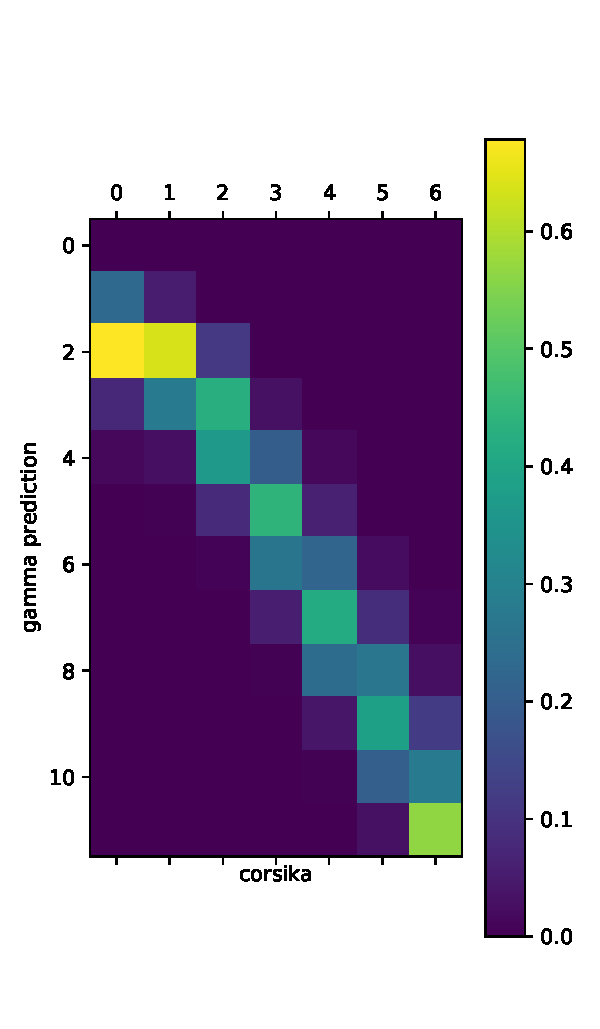
\includegraphics[width=0.5\textwidth]{plots/Matrix.pdf}
  \caption{The migrationmatrix of the random-forest regressor.}
  \label{fig:matrix}
\end{figure}

In Figure \ref{fig:Edist} the energy distributions for both the on-region and the off-region are displayed. 
It can be seen, that very few events are more energetic than $\SI{10}{\tera\electronvolt}$ so the 
"overflow bin" at $\SI{50}{\tera\electronvolt}$ is not that relevant but not negligable either.

\begin{figure}[H]
  \centering
  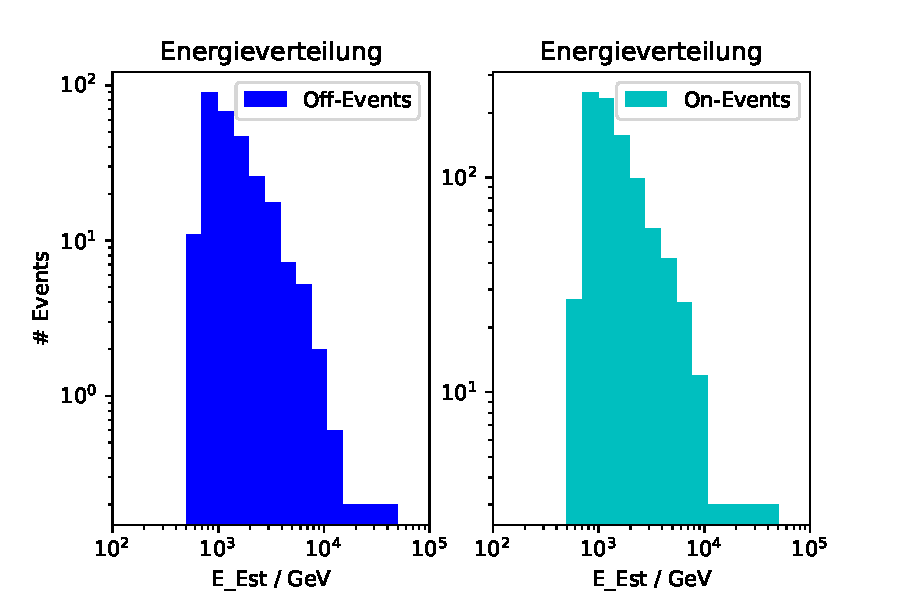
\includegraphics[width=0.8\textwidth]{plots/E_verteilung.pdf}
  \caption{energy distributions for on- and off-regions.}
  \label{fig:Edist}
\end{figure}

\subsubsection{Naive SVD unfolding}
Following equation \eqref{eqn:svd}, the histograms for the background $\symbf{b}$ is taken from the off-region events 
and the histogram for the estimated gamma-energies is yielded from the on-regions.
With \texttt{scipy} and \texttt{uncertainties} the speudoinverse matrix was calculated and the unfolded energies calculated as shown in figure \ref{fig:svdUnfold}.

\begin{figure}[H]
  \centering
  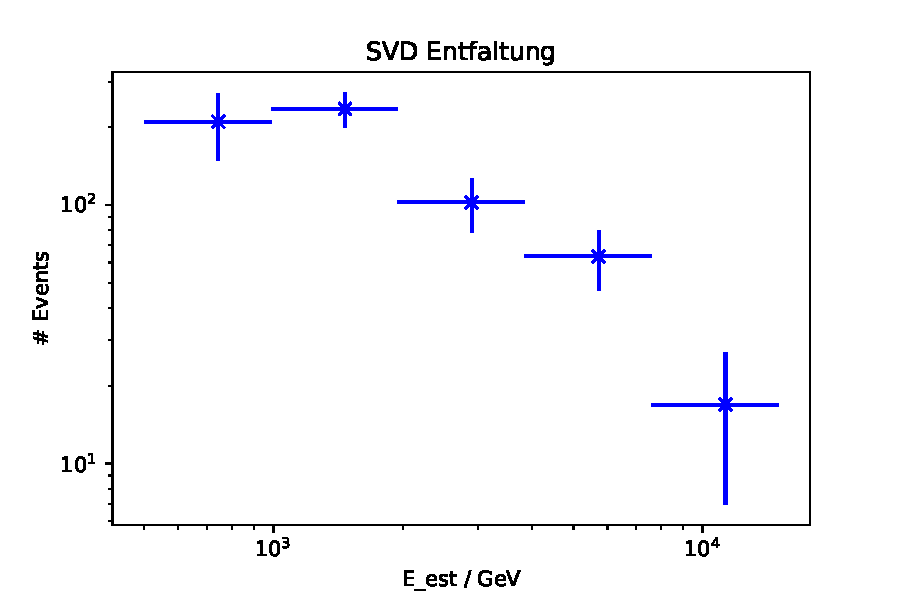
\includegraphics[width=0.8\textwidth]{plots/NSVD.pdf}
  \caption{unfolded energies with naive SVD.}
  \label{fig:svdUnfold}
\end{figure}

This unfolding method leads to an estimator for $\hat{\symbf{f}}$ of:

\begin{align}
\hat{\symbf{f}} &= 
\begin{pmatrix}
     210.21 \pm 60.88 \\
     235.61 \pm 36.74 \\
     102.47 \pm 24.21 \\
     63.46 \pm 16.53 \\ 
     16.90 \pm 9.94 \\
\end{pmatrix}
\end{align}


\subsubsection{Poisson-likelihood unfolding}
The poisson-likelihood unfolding was calculated using methods from \texttt{scipy}.
The minimization was done using the \texttt{L\-BFGS\-B} minimization 
function from \texttt{scipy\.optimize}.

In Figure \ref{fig:vgl} the poisson-likelihood unfolding 
is shown in blue and the naive SVD in red. 
They clearly show very similar results, therefore the flux 
can be calculated with unfolded data by any of these methods.

\begin{figure}[H]
\centering
\begin{subfigure}{0.45\textwidth}
  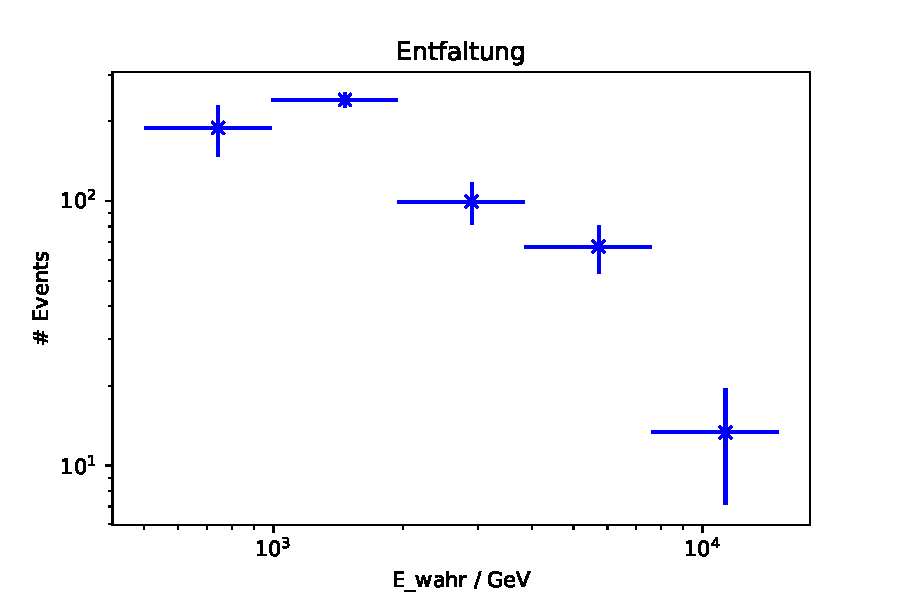
\includegraphics[width=\textwidth]{plots/Entfaltung_2.pdf}
  \caption{Unfolded data using poisson-likelihood unfolding.\label{fig:pois}}
\end{subfigure}
\begin{subfigure}{0.45\textwidth}
  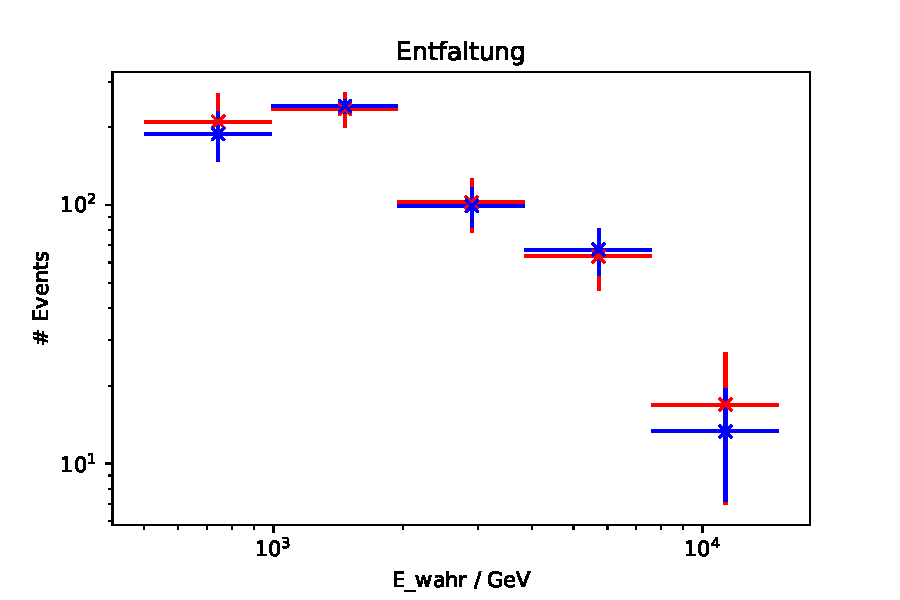
\includegraphics[width=\textwidth]{plots/Entfaltung_vgl.pdf}
  \caption{Comparison between both unfolding techniques.\label{fig:vgl}}
\end{subfigure}
\end{figure}

The poisson-likelihood method results in an esimator $\hat{\symbf{f}}$ of 

\begin{align}
\hat{\symbf{f}} &= 
\begin{pmatrix}
     188.75 \pm 40.98 \\
     241.08 \pm 15.70 \\
     99.47 \pm 17.74 \\
     67.21 \pm 13.92 \\ 
     13.37 \pm 6.24 \\
\end{pmatrix}
\end{align}

\subsection{Flux calculation}

The flux is calculated with
\begin{equation}
  \phi_i = \frac{\hat{f}_i}{A_{eff,i} \Delta\symup{E}_i t_{obs}}
  \label{eqn:flux}
\end{equation}
where $\Delta\symup{E}_i$ is the width of the energy bin, $t_{obs}$ is the duration of observation, $A_{eff,i}$ is calculated from
\begin{equation}
  A_{eff,i} = \frac{N_{selec, i}}{N_{sim, i}} \cdot A\,.
\end{equation}
The effective detector area is multiplied by $0.7$ since only $\SI{70}{\percent}$ of the data is taken.

The flux is calculated with the unfolded data both via both unfolding methods and shown in figure \ref{fig:fluxBoth}.
Both true-energies are pretty close together.

\begin{figure}[H]
  \centering
  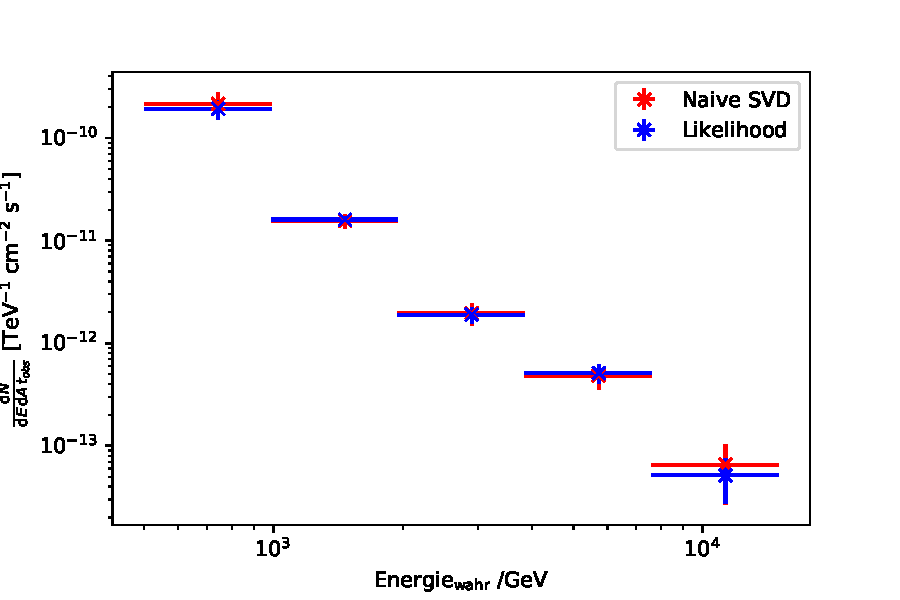
\includegraphics[width=0.8\textwidth]{plots/Fluss.pdf}
  \caption{flux calculation with naive SVD and poisson-likelihood against true-energy.}
  \label{fig:fluxBoth}
\end{figure}

\subsection{Comparison to HEGRA and MAGIC}

The fitting function used for the HEGRA and MAGIC data is defined as
\begin{equation}
  f(x, a, b, c, d) = a \left(\frac{x}{b}\right)^{\left(-c + d\cdot \ln\left(\frac{x}{b}\right)\right)}
\end{equation}
The parameters for both measurements are shown in table (to be made). The plot showing the comparison is shown in figure \ref{fig:fluxComp}.

Our analysis is compatible with the one of HEGRA and MAGIC for energies larger than $\SI{1}{\tera\electronvolt}$. The first value is slightly higher than in the other measurements but the scale is quite small, so is the error. Even for high energies our results are comparable to the ones from HEGRA. The flux calulated by MAGIC branches off of the HEGRA measurement but is still in agreement with our results.

\begin{figure}[H]
  \centering
  \includegraphics[width=0.8\textwidth]{plots/Fluss_like.pdf}
  \caption{Comparison of our flux measurements with HEGRA and MAGIC.}
  \label{fig:fluxComp}
\end{figure}
